\documentclass[8pt]{beamer}

\usepackage[utf8]{inputenc}
\usepackage{upquote}
\usepackage{graphicx}

\usetheme{Warsaw}

\AtBeginSection[]{
  \begin{frame}
  \vfill
  \centering
  \begin{beamercolorbox}[sep=8pt,center,shadow=true,rounded=true]{title}
    \usebeamerfont{title}
    \insertsectionhead\par%
    \vspace{2em}
  \end{beamercolorbox}
  \vfill
  \end{frame}
}

\AtBeginSubsection[]{
  \begin{frame}
  \vfill
  \centering
  \begin{beamercolorbox}[sep=8pt,center,shadow=true,rounded=true]{title}
    \usebeamerfont{title}
    \insertsectionhead\par%
    \vspace{1em}
    \insertsubsectionhead\par%
  \end{beamercolorbox}
  \vfill
  \end{frame}
}

\title{*BSD}
\author{Thomas de Grivel {\tt thoxdg@gmail.com}}
\institute{http://kmx.io}
\date{\today}

\begin{document}

\begin{frame}
\titlepage
\end{frame}

\section{UNIX}
\subsection{History}

\begin{frame}
  \frametitle{Diagram}
  \begin{figure}[h!]
    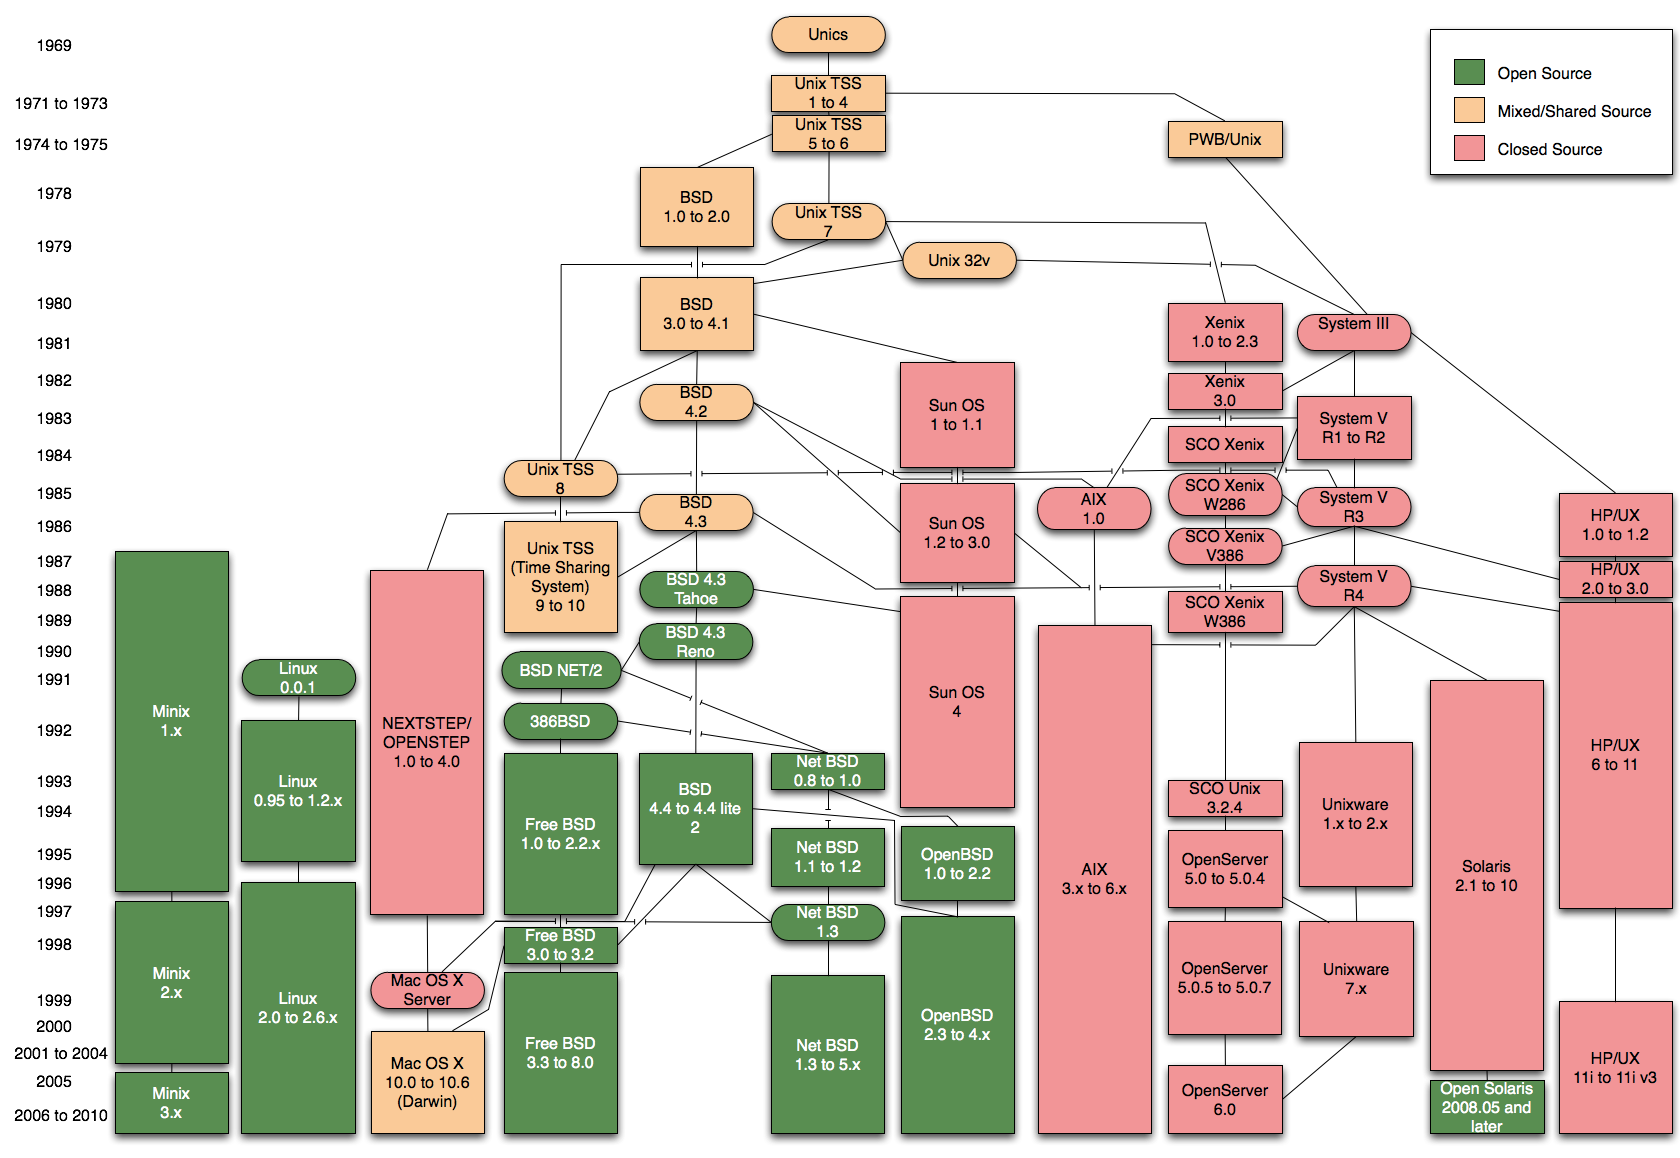
\includegraphics[width = 11cm]{unix-history.png}
    \label{UNIX}
  \end{figure}
\end{frame}

\begin{frame}
  \frametitle{Multics}
  1960\\
  \vspace{1em}
  Companies
  \begin{itemize}
  \item MIT
  \item AT\&T Bell labs
  \item General Electric
  \end{itemize}
  \vspace{1em}
\end{frame}

\begin{frame}
  \frametitle{UNIX}
  AT\&T Bell Labs 1970 \\
  \vspace{1em}
  Developers
  \begin{itemize}
  \item Ken Thompson
  \item Dennis Ritchie
  \end{itemize}
\end{frame}

\begin{frame}
  \frametitle{Berkeley Unix}
  1974 \\
  \vspace{1em}
  Licensed by AT\&T
\end{frame}

\begin{frame}
  \frametitle{Berkeley Software Distribution}
  1979 \\
  \vspace{1em}
  \begin{itemize}
  \item {\tt vi}
  \item {\tt csh}
  \end{itemize}
  \vspace{1em}
  Licensed by AT\&T
\end{frame}

\begin{frame}[fragile]
  \frametitle{BSD License}
\begin{verbatim}
Copyright (c) <year> <copyright holder>.
All rights reserved.

Redistribution and use in source and binary forms are permitted
provided that the above copyright notice and this paragraph are
duplicated in all such forms and that any documentation,
advertising materials, and other materials related to such
distribution and use acknowledge that the software was developed
by the <organization>. The name of the
<organization> may not be used to endorse or promote products derived
from this software without specific prior written permission.
THIS SOFTWARE IS PROVIDED ``AS IS'' AND WITHOUT ANY EXPRESS OR
IMPLIED WARRANTIES, INCLUDING, WITHOUT LIMITATION, THE IMPLIED
WARRANTIES OF MERCHANTABILITY AND FITNESS FOR A PARTICULAR PURPOSE.
\end{verbatim}
\end{frame}

\begin{frame}
  \frametitle{Net/1}
  June 1989 \\
  \vspace{1em}
  Basis for
  \begin{itemize}
  \item NetBSD
  \item FreeBSD
  \end{itemize}
  \vspace{1em}
  Under BSD License
\end{frame}

\begin{frame}
  \frametitle{Minix}
  Andrew S. Tannenbaum
  \begin{itemize}
  \item For teaching
  \item Not BSD
  \item GPL
  \end{itemize}
\end{frame}

\begin{frame}
  \frametitle{Linux}
  Linus Torvalds
  \begin{itemize}
  \item Inspired by Minix
  \item Not BSD
  \item GPL
  \end{itemize}
\end{frame}

\begin{frame}
  \frametitle{NetBSD}
  Computer Systems Research Group of the University of California, Berkeley
  \begin{itemize}
  \item Started in 1993 from Net/2 and 386BSD
  \item BSD License (two, three, and four-clause variants)
  \item {\bf Portable}
  \end{itemize}
  \vspace{1em}
  Founders :
  \begin{itemize}
  \item Chris Demetriou
  \item Theo de Raadt
  \item Adam Glass
  \item Charles Hannum
  \end{itemize}
\end{frame}

\begin{frame}
  \frametitle{FreeBSD}
  \begin{itemize}
  \item Started in 1993 also from 386BSD
  \item FreeBSD 2.0 in 1994, without code from AT\&T
  \item {\bf Fast} {\tt jemalloc} in base
  \end{itemize}
\end{frame}

\begin{frame}
  \frametitle{OpenBSD}
  Theo de Raadt
  \begin{itemize}
  \item forked from NetBSD in 1995
  \item {\bf Secure by default}
  \item Home of CARP, cwm, httpd, LibreSSL, OpenBGPD, OpenIKED, {\bf OpenNTPD}, OpenOSPFD, OpenRsync, OpenSMTPD, {\bf OpenSSH}, PF, pfsync, sndio, spamd, Xenocara
  \end{itemize}
\end{frame}

\begin{frame}
  \frametitle{Darwin}
  \begin{itemize}
  \item Forked from FreeBSD by Apple Inc. in 2000
  \item Includes code from NeXTSTEP and Mach
  \item Basis for MacOS X, iOS, iPadOS
  \item Apple Public Source License (APSL), with closed-source drivers
  \end{itemize}
\end{frame}

\end{document}
